\providecommand{\topdir}{..}
\documentclass[../main.tex]{subfiles}

%External sources
\graphicspath{{\topdir/img/04/}}

\begin{document}
\label{chap:desc}

The adopted solution can be divided into three parts. The first part relates to the low-level handling of video signals in the server. The second one is about the implementation of the server itself and the third one treats the client web application. Additionally, details about the implementation of the physical control panel prototype can be found in the \autoref{chap:control}.\newline

The parts regarding the server have been implemented using C++17 and they are meant to be run under Linux. However, no \gls{os}-specific libraries have been used, so it should work with any other \gls{os} with minor modifications. The web application has been implemented using the standard web development languages, namely \gls{html}, \gls{css} and \gls{js}. Therefore, there is no \gls{os} nor web browser limitation regarding it. Both pieces of software were developed using Microsoft's Visual Studio Code \gls{ide}.\newline

\section{Video manipulation library}

This section describes how low-level video data is handled by this software. To do so, it uses a video manipulation library called \textit{Zuazo} which is a  personal project of the author of this work. This software library allows to manipulate real-time video using \gls{gpu} acceleration though the \textit{Vulkan} graphics \gls{api}.\newline

\textit{Zuazo} is divided into multiple modules. A project may choose to include an arbitrary set of them. The modules used in this project are the following:

\begin{itemize}
    \item \textbf{zuazo}: Core functions for the library. Must be always included if any component of the library is used.
    \item \textbf{zuazo-compositor}: Video composition utilities.
    \item \textbf{zuazo-ndi}: \Gls{ndi} \gls{io}. Wraps NewTek's official \gls{ndi} library in a \textit{Zuazo} coherent interface.
    \item \textbf{zuazo-ffmpeg}: Compressed video input through the \textit{FFmpeg} library.
    \item \textbf{zuazo-window}: Window and monitor output the \textit{GLFW} library.
\end{itemize}


\subsection{RGB conversion pipeline}

Most image operations are intended to be performed in a linear \gls{rgb} color model. This means that the component values must be proportional to the tristimulus received by the camera. However, this signal is rarely used in transmission and storage. Therefore, all ingested signals are converted to an adequate \gls{pixel} format. The general conversion pipeline is shown in the figure \ref{fig:04:uploader}.\newline

\begin{figure}[htbp]
    \centering
    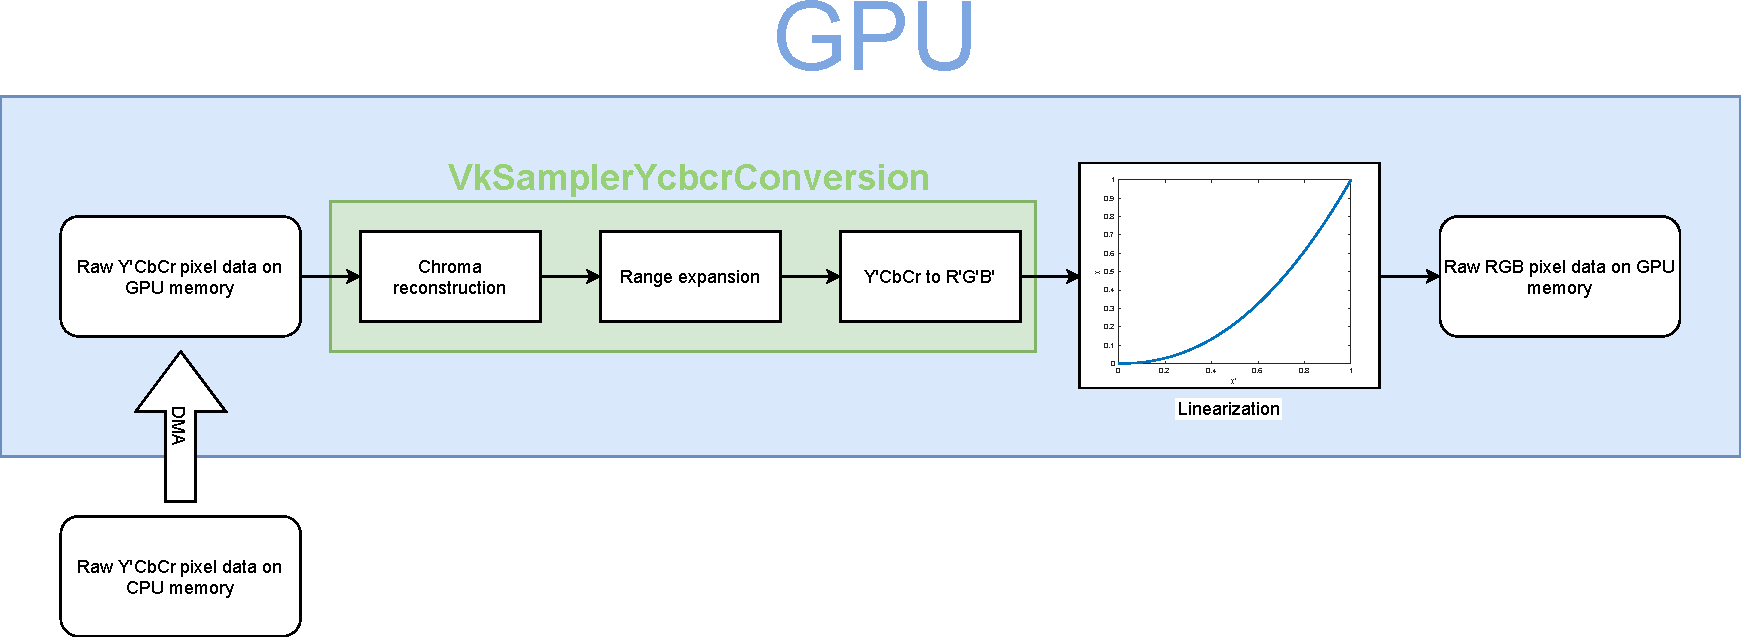
\includegraphics[width=\textwidth]{Uploader}

    \caption{Y'CbCr to RGB conversion pipeline}
    \label{fig:04:uploader}
\end{figure}

\subsubsection{Data upload}
Independently of the source of the video signal, the starting point of this process is \gls{cpu}'s memory, where the source has deposited raw \gls{pixel} data. This data may have an arbitrary bit-depth, multiplex, colour model, \gls{eotf}, etc\dots As the objective is to obtain raw linear \gls{rgb} data, this buffer is uploaded to another buffer that lies on the \gls{gpu}'s own memory. The \gls{gpu} is responsible of converting this untreated data to a easily manageable format. The data transfer is performed through a asynchronous \gls{dma} operation, so that the \gls{cpu} can handle other tasks meanwhile.


\subsubsection{Chroma reconstruction}
More often than not, when using Y'CbCr-like color models, chrominance components (Cb and Cr) are subsampled, this is, less values of them are stored, as shown in the figure \ref{fig:04:chroma_subsampling}. To represent this operation, the following notation is widely used: 

\begin{center}
    $<$luma samples on any line$>$:$<C_b, C_r$ samples on even lines$>$:$<C_b, C_r$ samples on odd lines$>$
\end{center}

\begin{figure}[htbp]
    \centering
    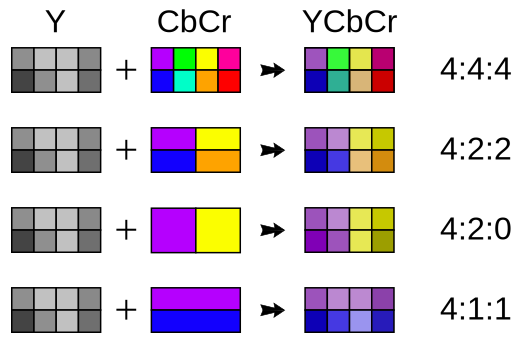
\includegraphics[width=.8\textwidth]{Chroma subsampling}

    Source: Wikipedia
    \caption{Common chroma subsampling schemes}
    \label{fig:04:chroma_subsampling}
\end{figure}

The following subsampling schemes are supported:

\begin{itemize}
    \item 4:4:4 (no subsampling)
    \item 4:2:2
    \item 4:2:0
    \item 4:1:1
    \item 4:1:0
    \item 3:1:1
    \item 3:1:0
\end{itemize}

Moreover, there are several ways of aligning the chroma sample grid with the luma sample grid. This alignment is also taken into account. Considering these two parameters, the chroma samples are linearly interpolated to match the luma sample count.


\subsubsection{Range expansion}

Due to legacy reasons, many video signals do not use the whole available range for their respective bit-depth. If this is the case, the components are expanded according to the ITU-R BT.601 standard\cite{bt601}. If an alpha channel is present, it may bypass this step, depending on the information provided by the source. The aforementioned range expansion is performed with the equation \eqref{eq:04:expansion_rgbay} for $R, G, B, A, Y \in [0, 1]$ components and with the equation \eqref{eq:04:expansion_cbcr} for $C_b, C_r \in [-0.5, +0.5]$, where $n$ is the bit-depth.\newline

\begin{equation}\label{eq:04:expansion_rgbay}
    Y' = \frac{y' \cdot (2^n - 1) - 16\cdot2^{n-8}}{219 \cdot 2^{n-8}}
\end{equation}

\begin{equation}\label{eq:04:expansion_cbcr}
    C' = \frac{c' \cdot (2^n - 1)}{224 \cdot 2^{n-8}}
\end{equation}


\subsubsection{Colour model conversion}

If using a Y'CbCr-like colour model, this needs to be converted to R'G'B' (gamma corrected \gls{rgb}). This is a simple linear transformation that is performed using a 3x3 matrix. The values of the matrix depend on the actual Y'CbCr specification. Obviously, if the source data is in \gls{rgb} space, no conversion will be performed. \newline

The following Y'CbCr specifications are supported:

\begin{itemize}
    \item RGB (no conversion)
    \item YIQ
    \item YUV
    \item ITU-R BT.601\cite{bt601}
    \item ITU-R BT.709\cite{bt709}
    \item ITU-R BT.2020\cite{bt2020}
    \item SMPTE 240M\cite{smpte240M}
\end{itemize}


If \textit{Vulkan} supports the \texttt{VkSamplerYcbcrConversion} extension and this extension supports the requested configuration, the last three operations are executed by \textit{Vulkan} itself. Otherwise, a fallback method that performs them on a fragment shader is available. Moreover, partially supported configurations may also take advantage of the extension.\newline

\subsubsection{Component linearization}

The last step is to linearize the inverse \gls{eotf} applied to the \gls{pixel} data. This is done because mixing gamma-corrected values leads to colorimetrically incorrect results. Alpha component bypasses this stage, as it is not gamma corrected.\newline

The following \glspl{eotf} are supported:

\begin{itemize}
    \item Linear (no linearization needed)
    \item ITU-R BT.1886\cite{bt1886}
    \item Gamma 2.2
    \item Gamma 2.6
    \item Gamma 2.8
    \item IEC61966-2-1\cite{iec61966-2-1}
    \item IEC61966-2-4\cite{iec61966-2-4}
    \item SMPTE 240M\cite{smpte240M} 
    \item SMPTE ST.2084\cite{smpte2084}
    \item ARIB STD-B67\cite{aribStdB67}
\end{itemize}

The resulting RGB(A) image is stored on a \textit{Vulkan} texture local to the \gls{gpu} memory. All components are represented by floating-point numbers whose mantissa has more bits than the source component. In other words, if the source format has strictly less than 12 bits per component, a 16 bit floating-point (half precision) number will be used. Otherwise, 32 bits (single precision) will be used\cite{ieee754}.\newline

There are some exceptional cases where the aforementioned conversions are not performed. For those cases, the data is copied directly from the \gls{cpu} to the definitive \gls{gpu} buffer, preserving the original pixel format. These exceptions are the following:

\begin{enumerate}[label=(\alph*)]
    \item Source data is full-range RGB(A) with no gamma correction. After all, none of the stages would be executed.
    \item Source data is full-range RGB(A), with 8bits per component, IEC61966-2-1 encoding and \textit{Vulkan} supports sRGB formats. In this case, all operations except the linearization are a no-op. When sRGB formats are supported, this linearization is performed on the \gls{tmu} of the \gls{gpu} each time the texture is accessed.
\end{enumerate}

The reverse pipeline has been partially implemented, but none of the features provided by this mixer make extensive use of it.\newline



\subsection{Video processing}
Once a manageable video frame is on \gls{gpu} memory, it is considered to be a texture. In the context of computer graphics, textures are the basic form of interpreting image data on \glspl{gpu}. These textures are mapped to objects in a process known as UV-mapping. For this application, the whole texture will be assigned to a rectangle object.\newline

This presents a new problem. If the aspect ratio of the rectangle does not match the aspect ratio of the frame, special consideration needs to be taken. Several solutions have been implemented and it is up to the user to choose one of them:

\begin{itemize}
    \item \textbf{Stretch}: The image will be distorted to fit the new aspect ratio.
    \item \textbf{Box}: The image will be resized by the most restrictive axis. 
    \item \textbf{Crop}: The image will be resized by the least restrictive axis.
    \item \textbf{Clamp horizontally}: The image will be resized by the horizontal axis. 
    \item \textbf{Clamp vertically}: The image will be resized by the vertical axis.
\end{itemize}

Another aspect regarding the textures is the sampling. When the aforementioned rectangle is rendered, each of its \glspl{pixel} will have to be assigned a color. This color comes from the texture, but it may not correspond to a intermediary position between \glspl{texel}. Therefore, neighbouring \glspl{texel} need to be interpolated to obtain the actual color. This interpolation must be performed with linear color values. Luckily, in the previous section, this premise was ensured. The interpolation techniques illustrated in the figures \ref{fig:04:texture_sampling1} and \ref{fig:04:texture_sampling2} have been implemented.\newline

\begin{figure}[htbp]
    \centering
    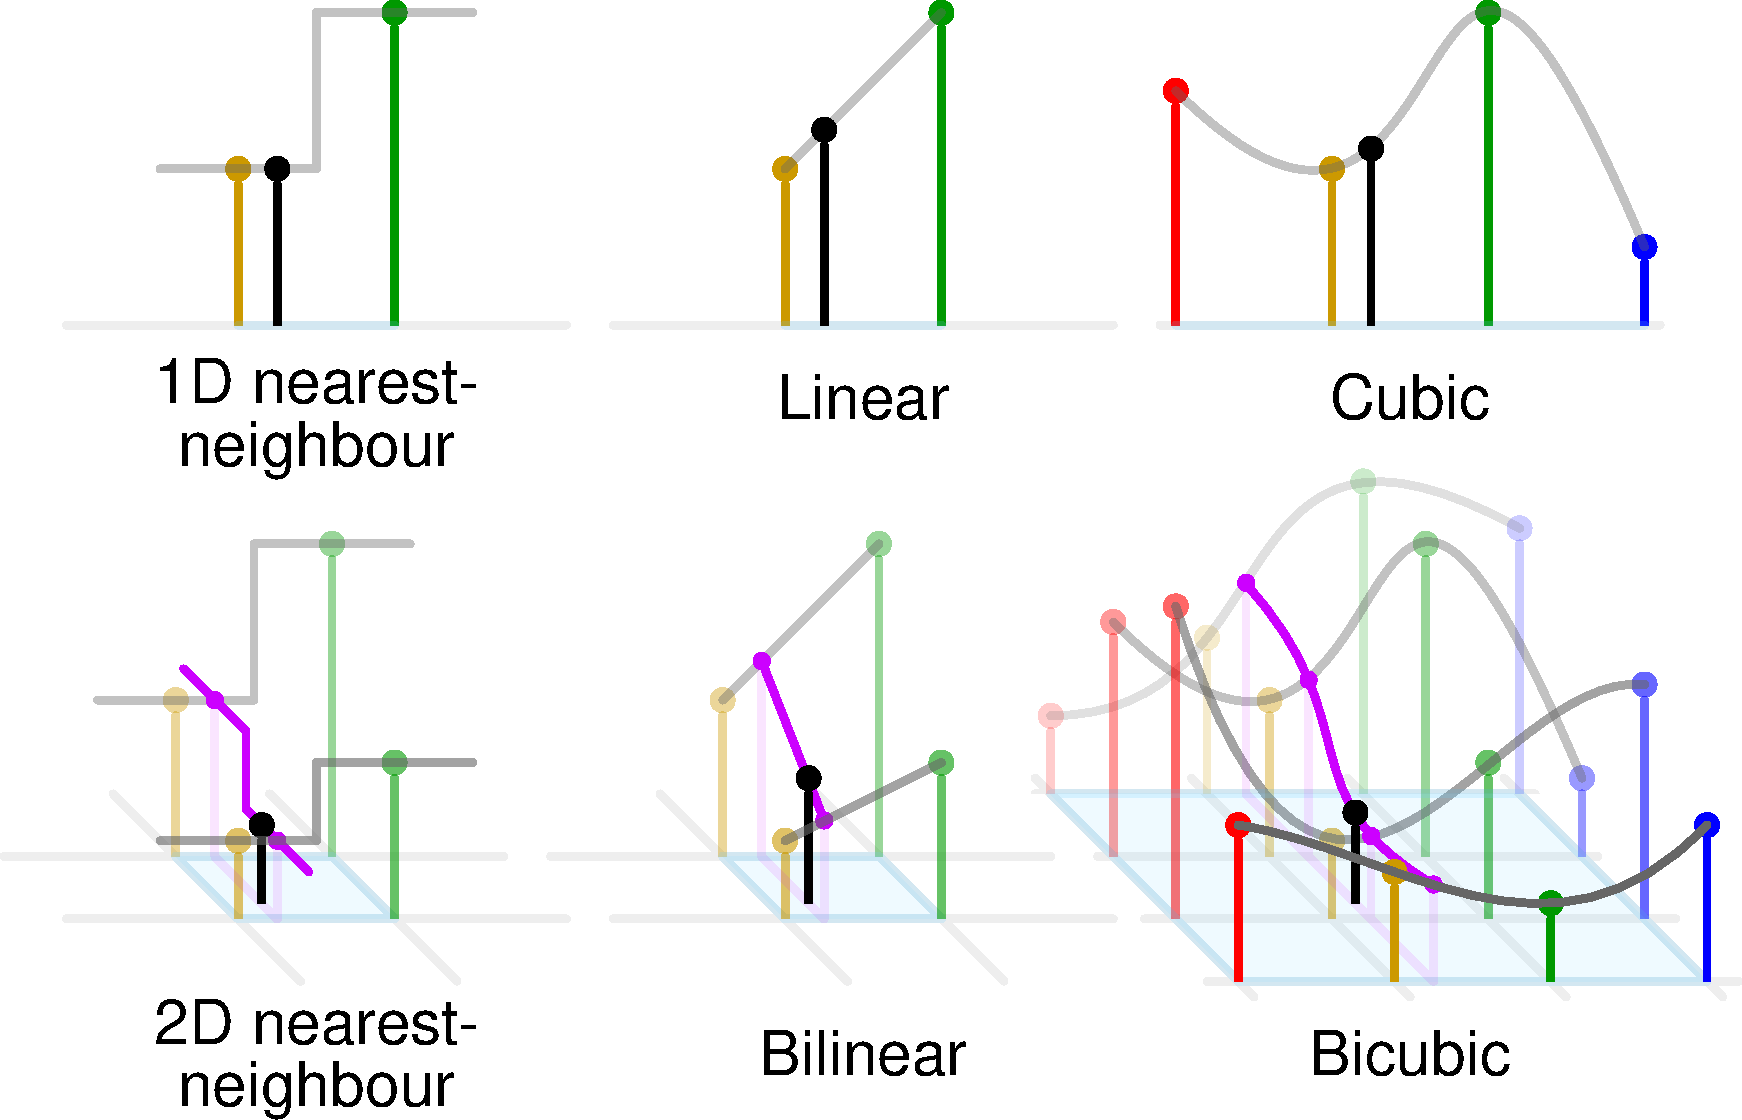
\includegraphics[width=\textwidth]{Interpolation}
    
    Source: Wikipedia
    \caption{Interpolation filters}
    \label{fig:04:texture_sampling1}
\end{figure}

\begin{figure}[htbp]
    \centering
    \subfigure[Nearest]{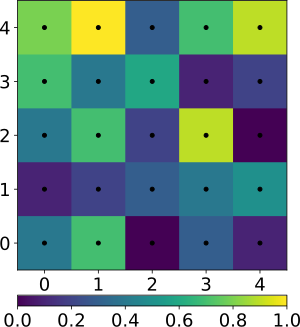
\includegraphics[width=.3\textwidth]{Interpolation-Nearest}}
    \subfigure[Bilinear]{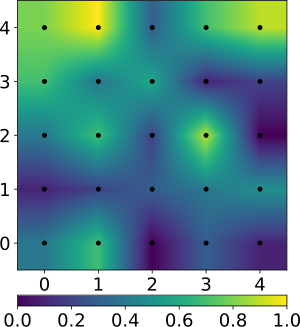
\includegraphics[width=.3\textwidth]{Interpolation-Bilinear}}
    \subfigure[Bicubic]{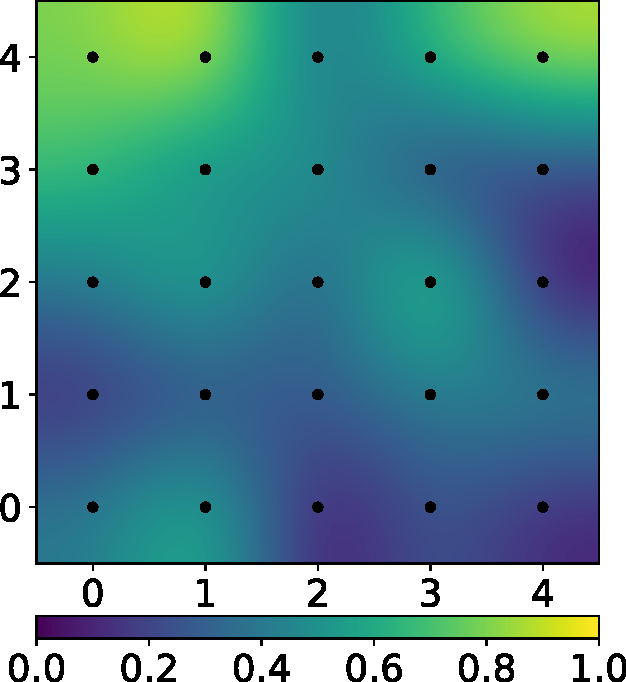
\includegraphics[width=.3\textwidth]{Interpolation-Bicubic}}
    
    Source: Wikipedia
    \caption{Texture sampling filters}
    \label{fig:04:texture_sampling2}
\end{figure}

Using nearest filtering is the cheapest option, as it requires a single texture access per sample. Bilinear filtering requires 4 accesses and 16 for bicubic filtering. Therefore, the later one is the costliest one and should not be used indiscriminately.\newline

From the implementation point of view, nearest filtering is always preformed by \textit{Vulkan}. In most cases, bilinear filtering is also executed by \textit{Vulkan} natively, but if this is not possible, a manual fallback method exists that implements it using 4 nearest accesses. Lastly, \textit{Vulkan} rarely supports bicubic filtering, but if this is the case, the \texttt{VK\_IMG\_filter\_cubic} extension is used. For the rest of the cases, it is implemented through 16 nearest accesses or 4 bilinear accesses. The later technique is based on a publicly available algorithm\cite{bicubicGlsl}.\newline

The resulting object is embedded into the framebuffer, the memory area where the \gls{gpu} works on. If the object presents transparency information, either because the original frame does or the processing has added to it, it will be blended with the existing contents in the framebuffer according to one of the following compositing modes. An example of each one of them can be seen in the figure \ref{fig:04:blending_modes}

\begin{itemize}
    \item \textbf{Write}: The framebuffer will be overwritten without considering its contents: $C = C_{object} \cdot \alpha$
    
    \item \textbf{Opacity}: Weighted average of the foreground and background colours. It is the most common blending mode: $C = C_{object} \cdot \alpha + C_{framebuffer} \cdot (1 - \alpha)$
    
    \item \textbf{Add}: Additive blending. The resulting value may be saturated: $C = C_{object} \cdot \alpha + C_{framebuffer}$
    
    \item \textbf{Inverse difference}: Subtracts the object's value to the existing colour. Useful to perform comparisons $C = C_{framebuffer} - C_{object} \cdot \alpha$
    
    \item \textbf{Difference}: Subtracts the existing value to the object's colour. Useful to perform comparisons: $C = C_{object} \cdot \alpha - C_{framebuffer}$
    
    \item \textbf{Darken}: The resulting colour will have the darkest components of the foreground and the background: $C = min\{C_{object} \cdot \alpha, C_{framebuffer}\}$
    
    \item \textbf{Lighten}: The resulting colour will have the brightest components of the foreground and the background: $C = max\{C_{object} \cdot \alpha, C_{framebuffer}\}$

    \item \textbf{Multiply}: The resulting colour will be the multiplication of the foreground and the background: $C = C_{object} \cdot \alpha \cdot C_{framebuffer}$
    
    \item \textbf{Screen}: Multiplication of complementary values: $1 - C = (1 - C_{object} \cdot \alpha) \cdot (1 - C_{framebuffer}) \Leftrightarrow C = C_{object} \cdot \alpha + C_{framebuffer} \cdot (1 - C_{object} \cdot \alpha)$
\end{itemize}

\begin{figure}[htbp]
    \centering
    \subfigure[Background]{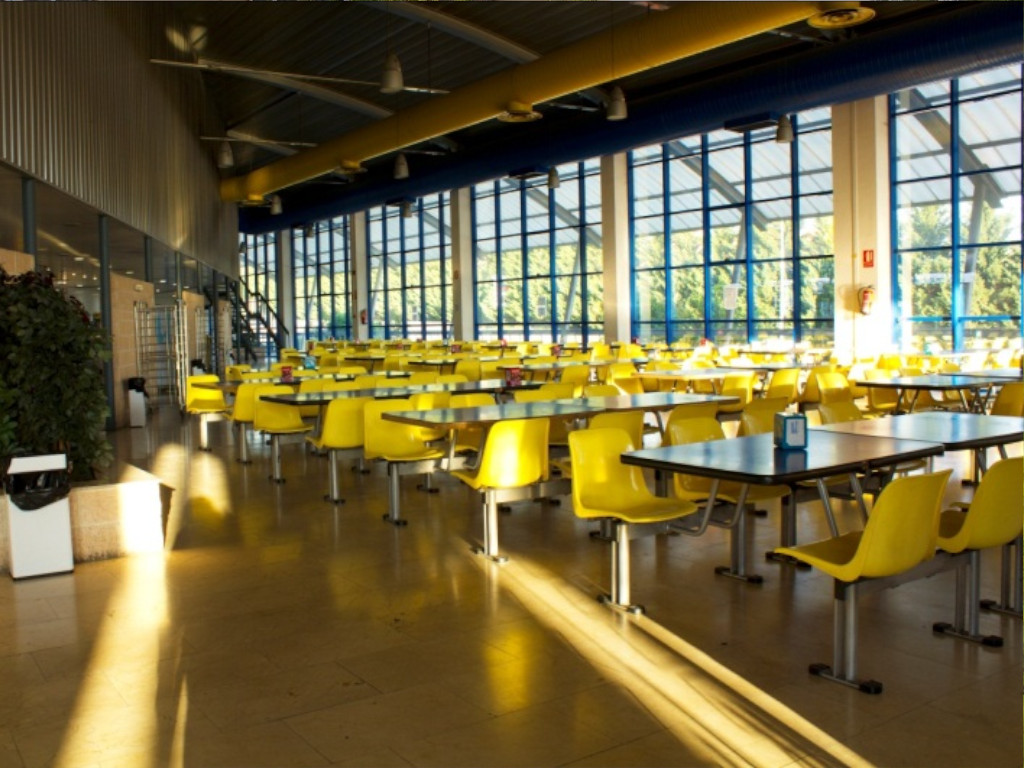
\includegraphics[width=.45\textwidth]{Blending mode-Background}}
    \subfigure[Foreground]{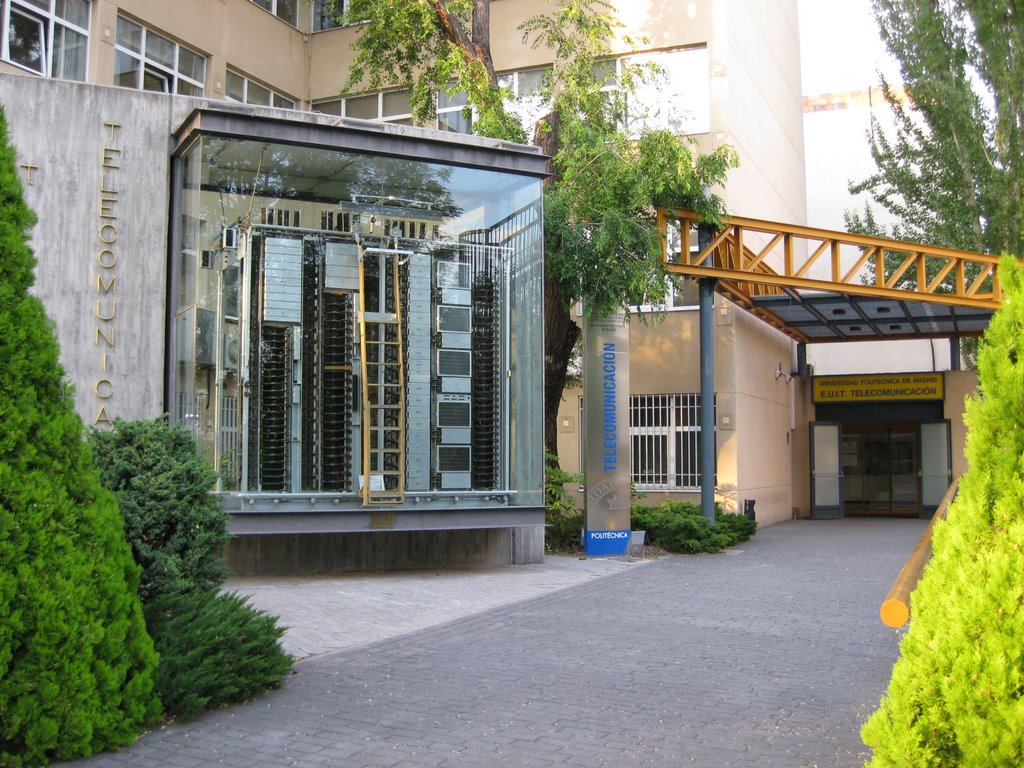
\includegraphics[width=.45\textwidth]{Blending mode-Foreground}}
    \subfigure[Write]{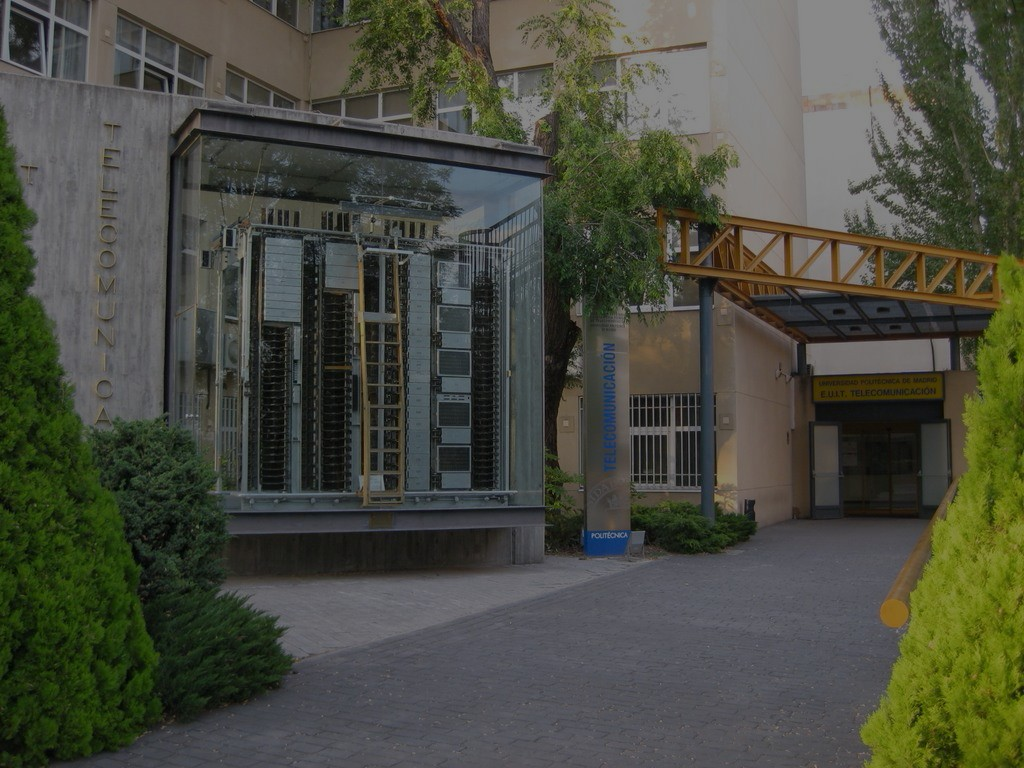
\includegraphics[width=.3\textwidth]{Blending mode-Write}}
    \subfigure[Opacity]{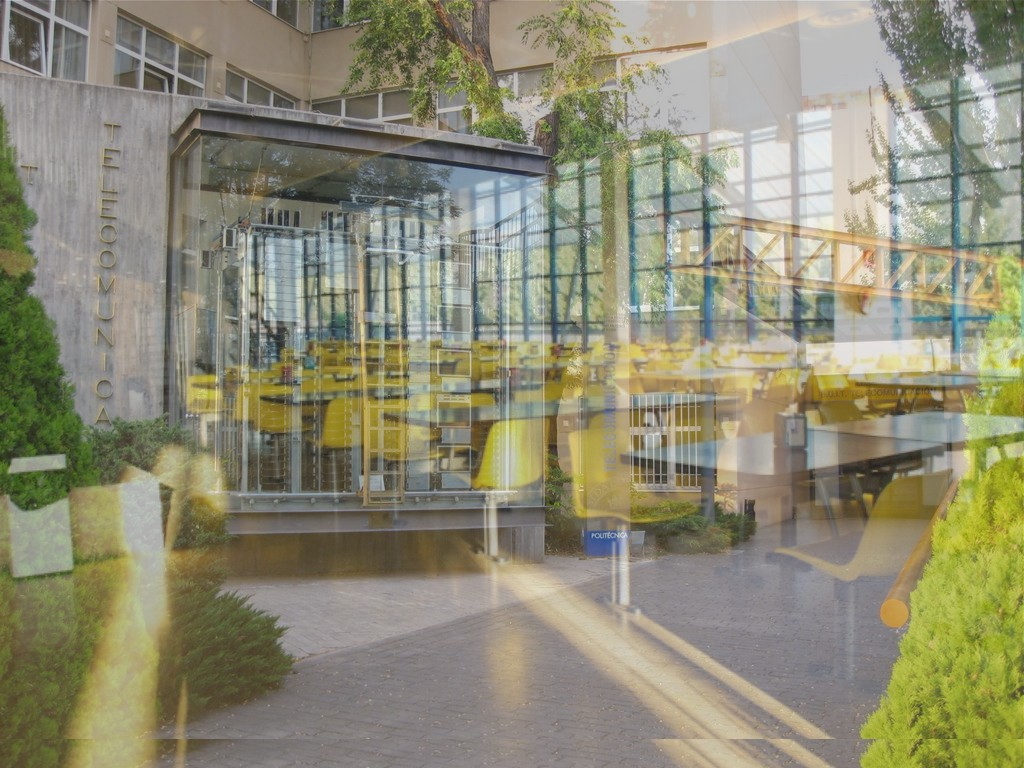
\includegraphics[width=.3\textwidth]{Blending mode-Opacity}}
    \subfigure[Add]{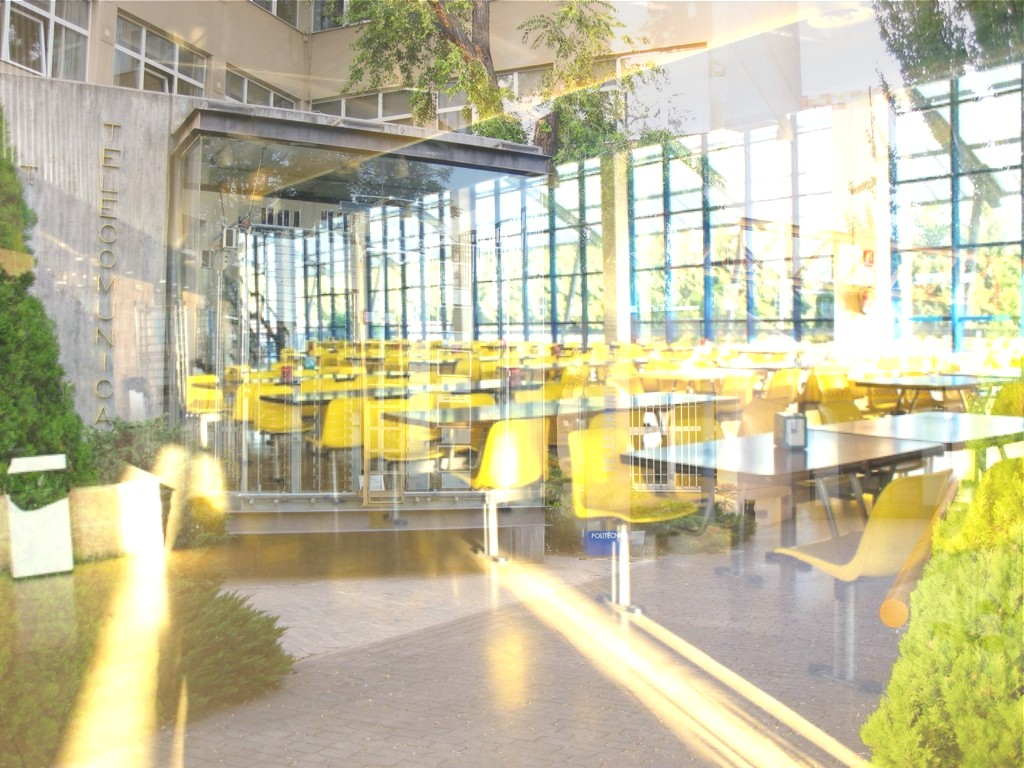
\includegraphics[width=.3\textwidth]{Blending mode-Add}}
    \subfigure[Inverse difference]{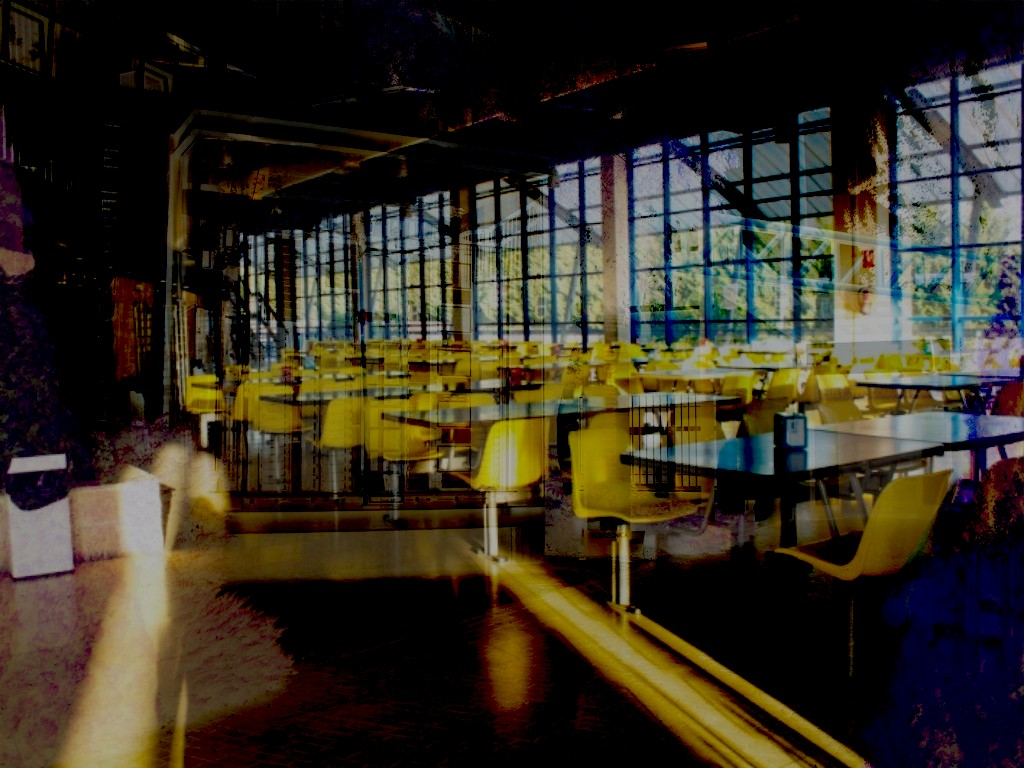
\includegraphics[width=.3\textwidth]{Blending mode-Difference1}}
    \subfigure[Difference]{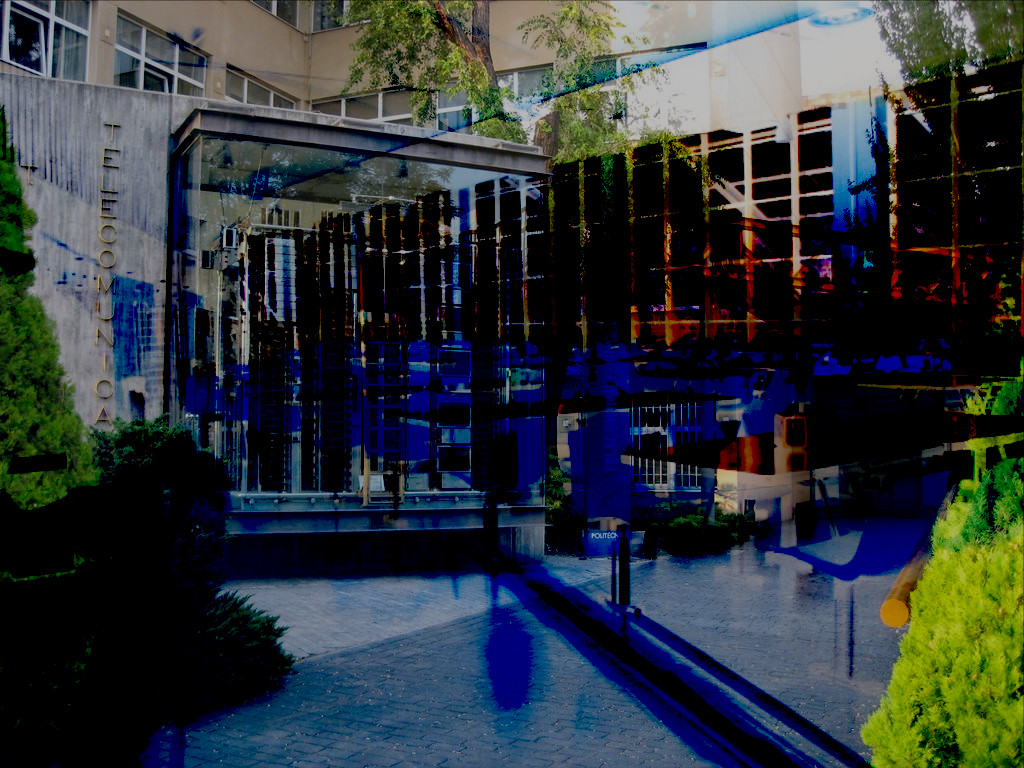
\includegraphics[width=.3\textwidth]{Blending mode-Difference}}
    \subfigure[Darken]{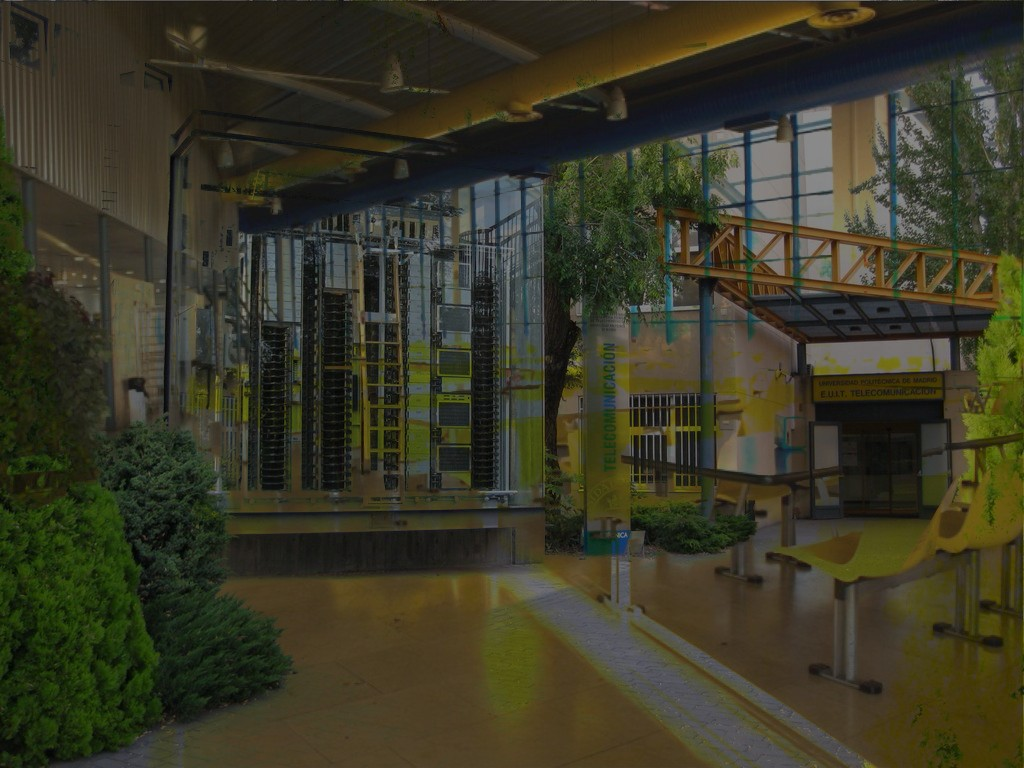
\includegraphics[width=.3\textwidth]{Blending mode-Darken}}
    \subfigure[Lighten]{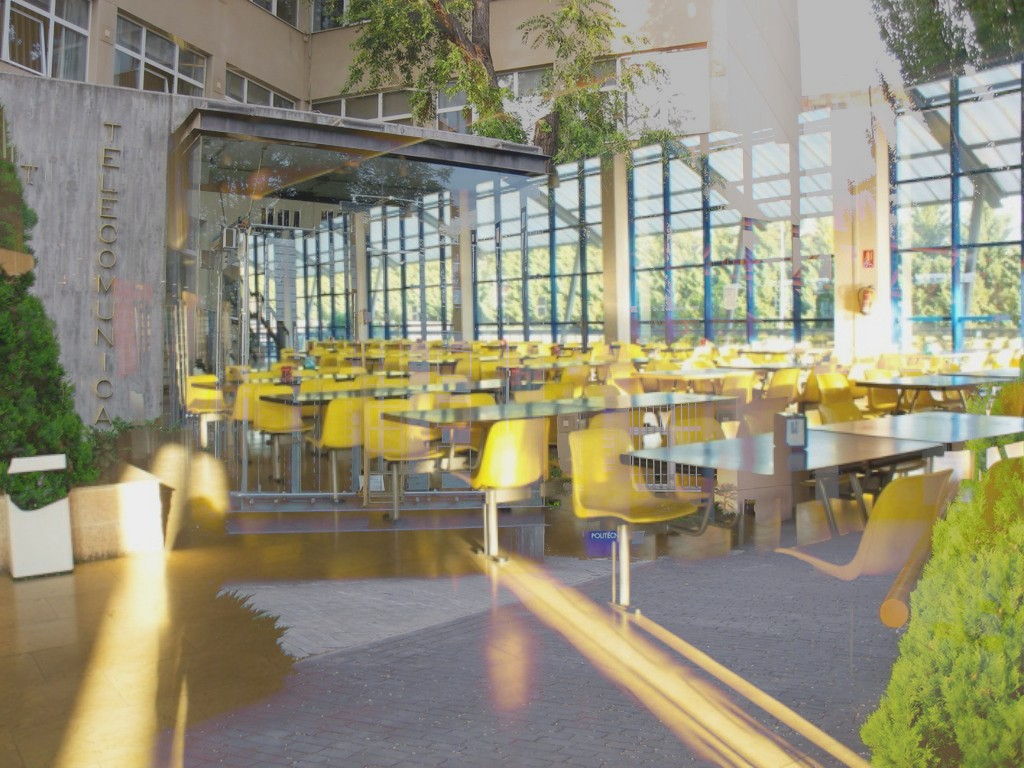
\includegraphics[width=.3\textwidth]{Blending mode-Lighten}}
    \subfigure[Multiply]{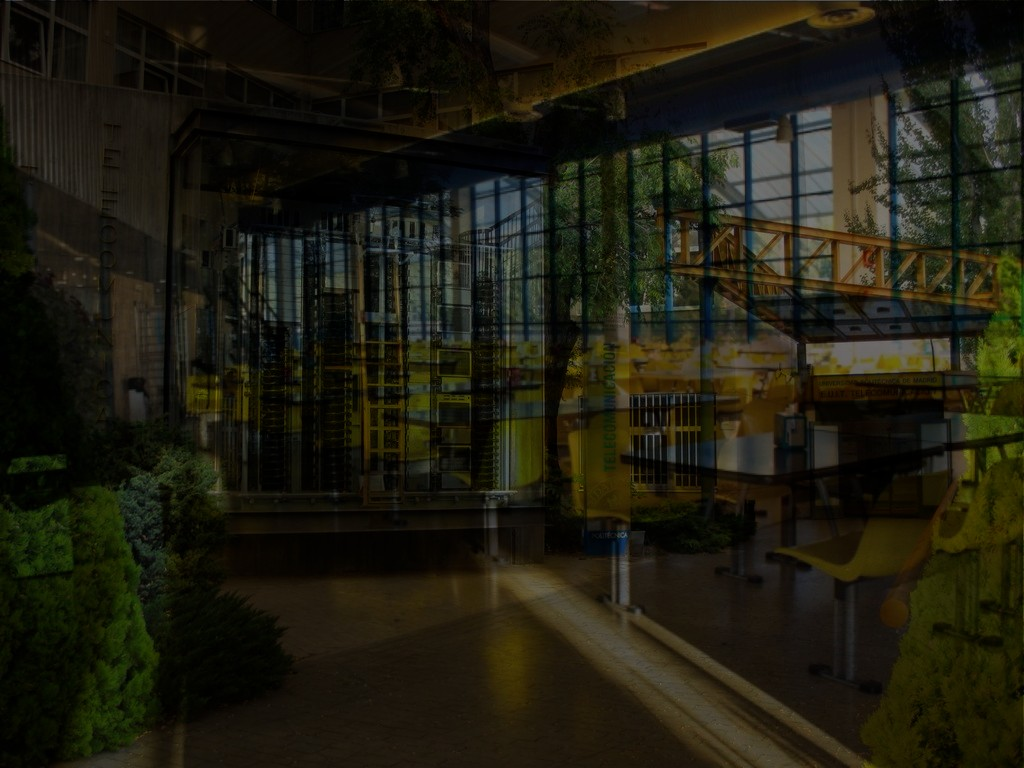
\includegraphics[width=.3\textwidth]{Blending mode-Multiply}}
    \subfigure[Screen]{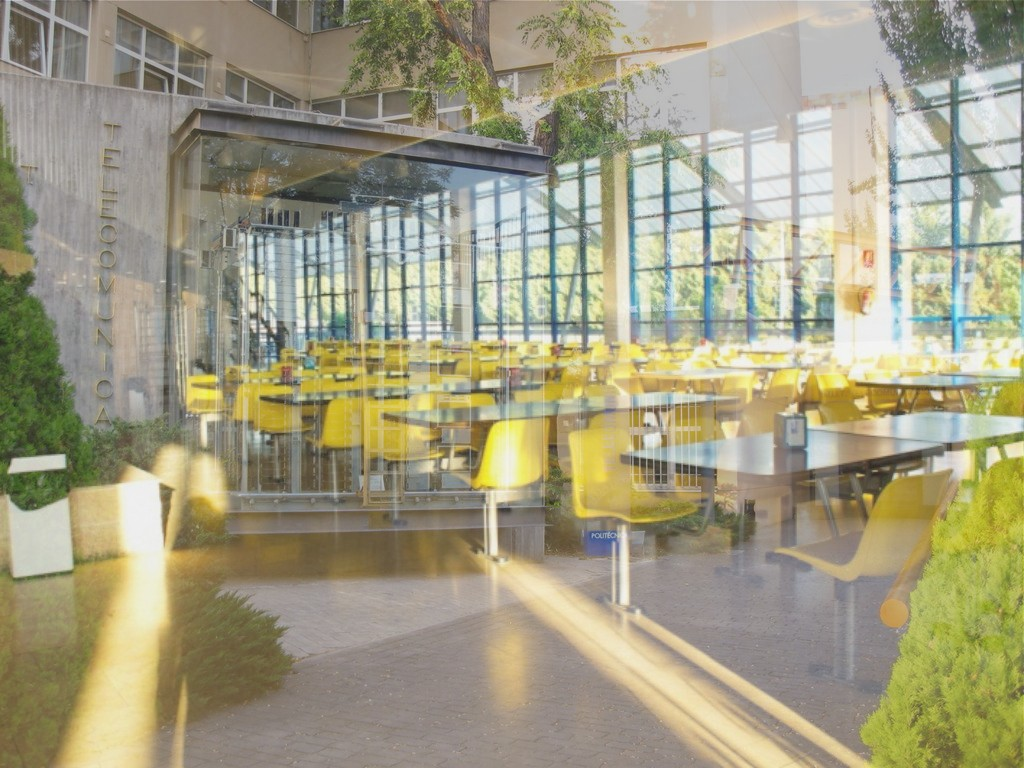
\includegraphics[width=.3\textwidth]{Blending mode-Screen}}

    \caption{Results of performing the blending operation with $\alpha=0.5$ and all supported modes.}
    \label{fig:04:blending_modes}
\end{figure}



\section{Server and communications}
The server itself has been developed using the previously described libraries. This server makes use of them to expose a \gls{cli} that resembles a vision mixer.\newline

This mixer is able to take live video feeds from \gls{ndi} sources or pre-recorded video files. Several heterogeneous \glspl{me} can be configured to manipulate those sources. Moreover, these \glspl{me} can be configured with arbitrary video parameters, such as nonstandard resolutions. The resulting video feeds can be outputted through a \gls{os} window or used as an input for other \glspl{me}. The windows can be configured to be full-screen on a monitor attached to the host computer, being able to use the video outputs of the computer.\newline

\subsection{Architecture}
The relations among the most crucial classes of the mixer have been illustrated in the figure \ref{fig:04:server_architecture}. A brief explanation about the duty of each one of the classes shown in this figure is described hereunder. The architecture can be divided into two parts. The first one relates to the infrastructure needed to configure the video manipulation. This includes all the classes owned by the Mixer class. The other part relates to the control of the former classes, this is, the classes owned by the Controller class.\newline

The mixer has been architected to allow easy expansion of both parts. This expansion can be done by defining new classes that inherit from the base classes.\newline

\begin{figure}[htbp]
    \centering
    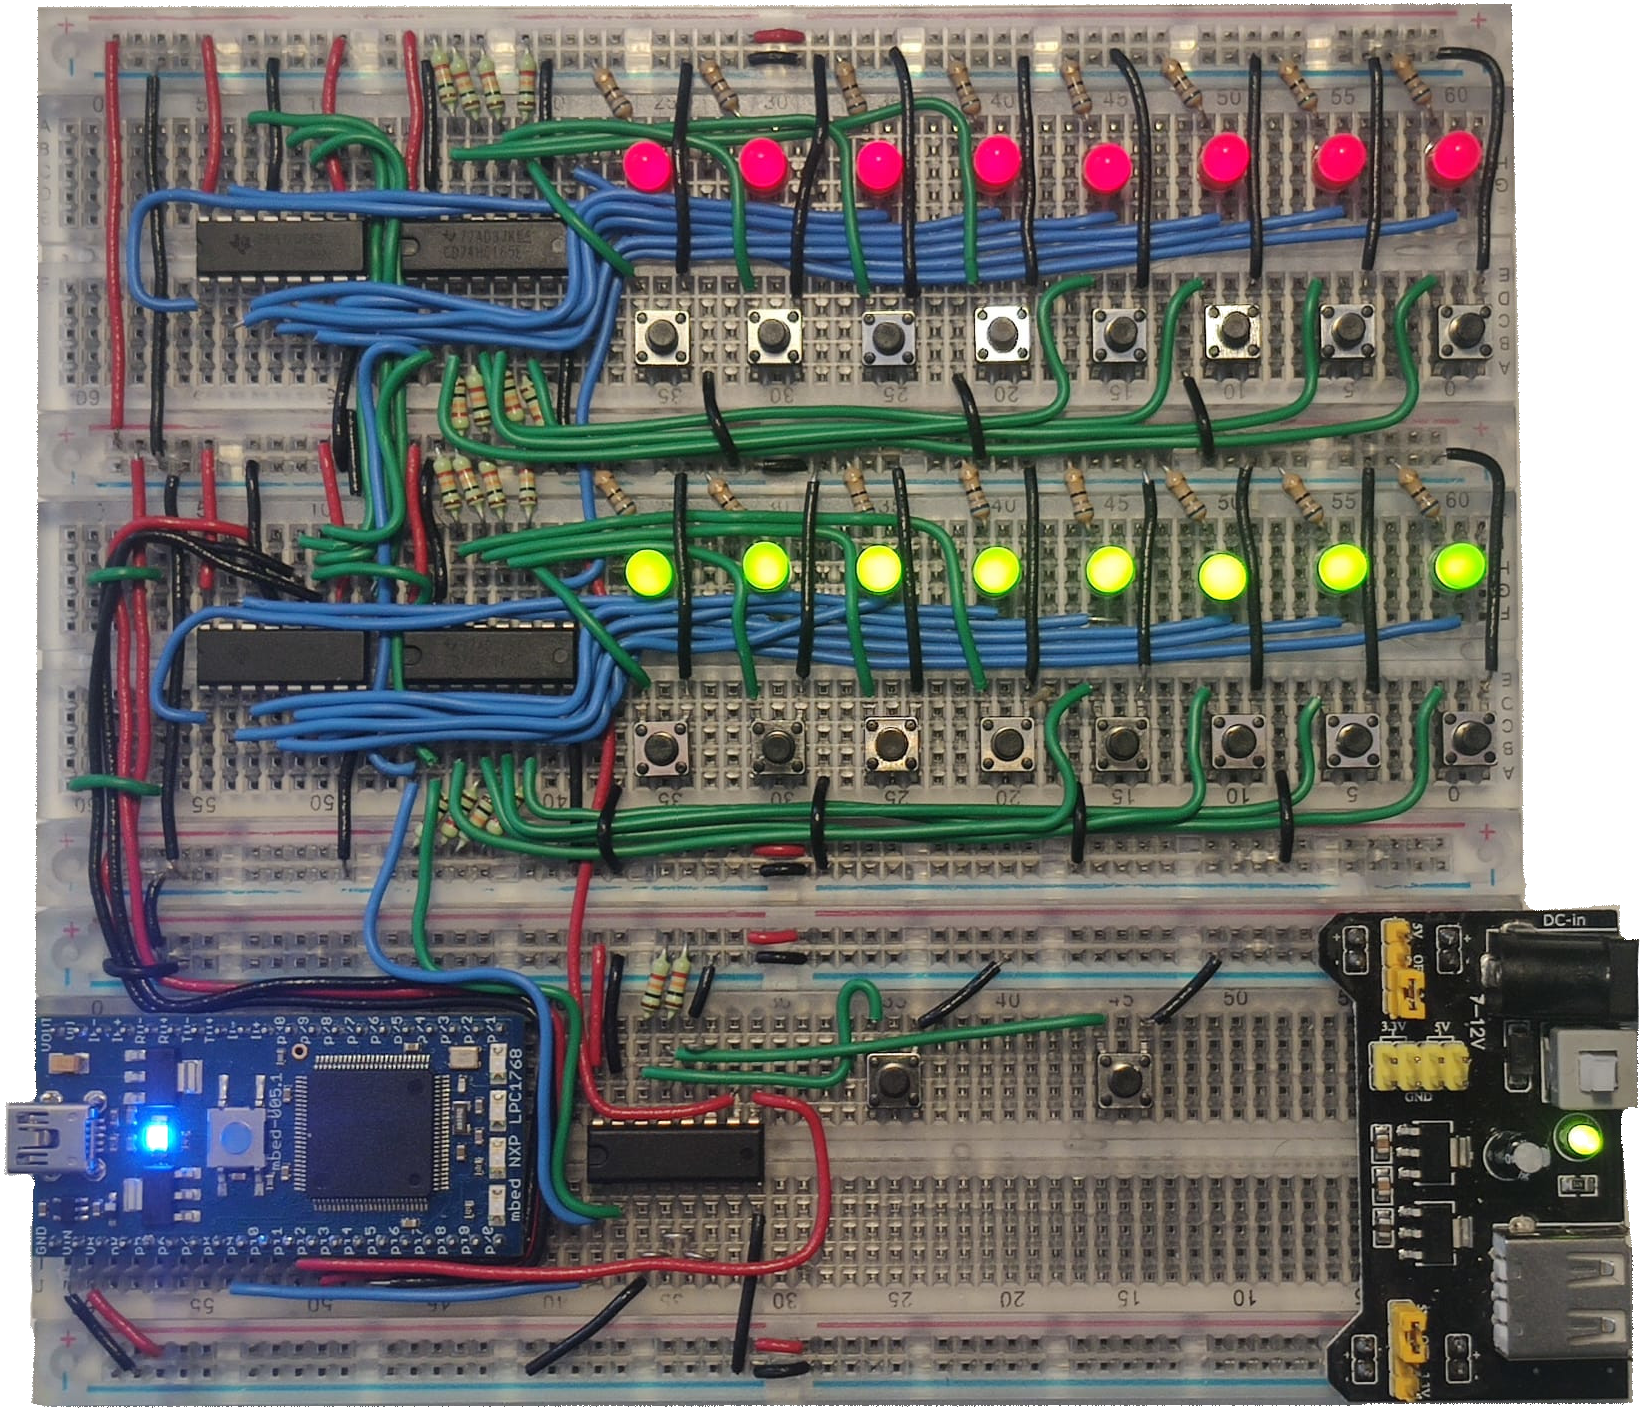
\includegraphics[width=\textwidth]{Cenital}

    \caption{Software architecture of the server side of the mixer}
    \label{fig:04:server_architecture}
\end{figure}

\subsubsection{Mixer}
The primary purpose of this class is to hold all elements that in some way interact with video signals. This includes inputs, outputs and \gls{me} banks. These elements can be dynamically constructed/destroyed on demand. They are held in a hash table where the key is provided by the unique name assigned to each of the elements. Moreover, it also serves as a signal matrix, as it has methods to route any output of any element to one of the inputs of another element. 

\subsubsection{ZuazoBase}
Strictly speaking, this class belongs to the \textit{Zuazo} library, but it is described here because it serves as the base class for all the classes regarding video manipulation. The hash table of the previous element holds instances of this class.

\subsubsection{Sources::NDI}
This class provides a \gls{ndi} source as a input for the mixer. The one available \gls{ndi} feeds is selected as the source.

\subsubsection{Sources::MediaPlayer}
Similarly to the mixer class, this class holds a hash indexed list of pre-recorded video clips. One of those clips is selected to be in the output. New clips can be loaded/unloaded dynamically.

\subsubsection{FFmpegClip}
These is the class held by the MediaPlayer class. It holds all the infrastructure needed to play a pre-recorded video file using the \textit{FFmpeg} library. This library is very versatile and allows to play almost all imaginable video containers and codecs. If possible, it will take advantage of hardware video decoding acceleration.\newline

The wrapper of this library provided by \textit{zuazo-ffmpeg} allows to set different repeat modes, play speeds, etc\dots

\subsubsection{Consumers::Window}
This class allows to create a window for showing video. This window can be configured to be full-screen on a monitor connected to the computer. Moreover, several other parameters such as window decoration, opacity and resizability can be tweaked.

\subsubsection{MixEffect}
Currently, this is the only class that manipulates video. The video compositing is performed using four instances of the \texttt{Compositor} component from the \textit{zuazo-compositor} module.\newline

As shown in the figure \ref{fig:04:compositing_no_transition}, generally, only two of the compositors are used, one for each output bus. These compositors render the background with all the overlays on top. Indeed, the overlays are ordered according to their priority, this is, high indexed overlays occlude lower indexed ones and \glspl{dsk} occlude \glspl{usk}.\newline

\begin{figure}[htbp]
    \centering
    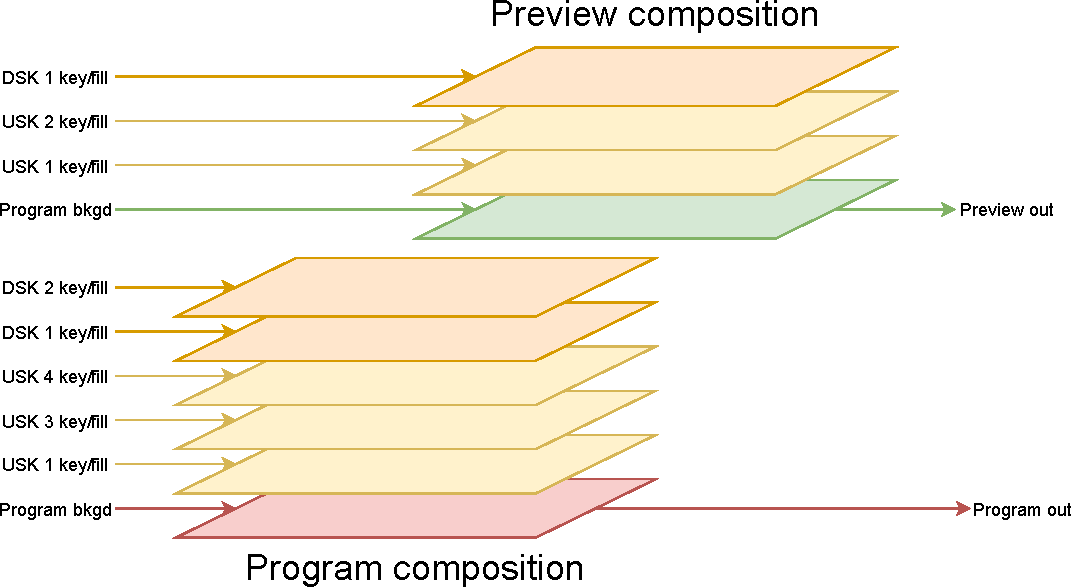
\includegraphics[width=\textwidth]{Mix effect-No transition}

    Layer legend: \textcolor{red}{Program background} \textcolor{green}{Preview background} \textcolor{yellow}{\glspl{usk}} \textcolor{orange}{\glspl{dsk}}
    \caption{Compositing layers when no transition is in progress}
    \label{fig:04:compositing_no_transition}
\end{figure}

However, if a transition is in progress, this behaviour changes, as \glspl{dsk} must be applied after the transition. Therefore, the other two compositors are used to generate a intermediate image that contains the background with all the \glspl{usk}. Both program and preview intermediate images are used to generate the transition on the configured output bus, as displayed in the figure \ref{fig:04:compositing_transition}. The other output bus is also composited but without the transition effect.

\begin{sidewaysfigure}[htbp]
    \centering
    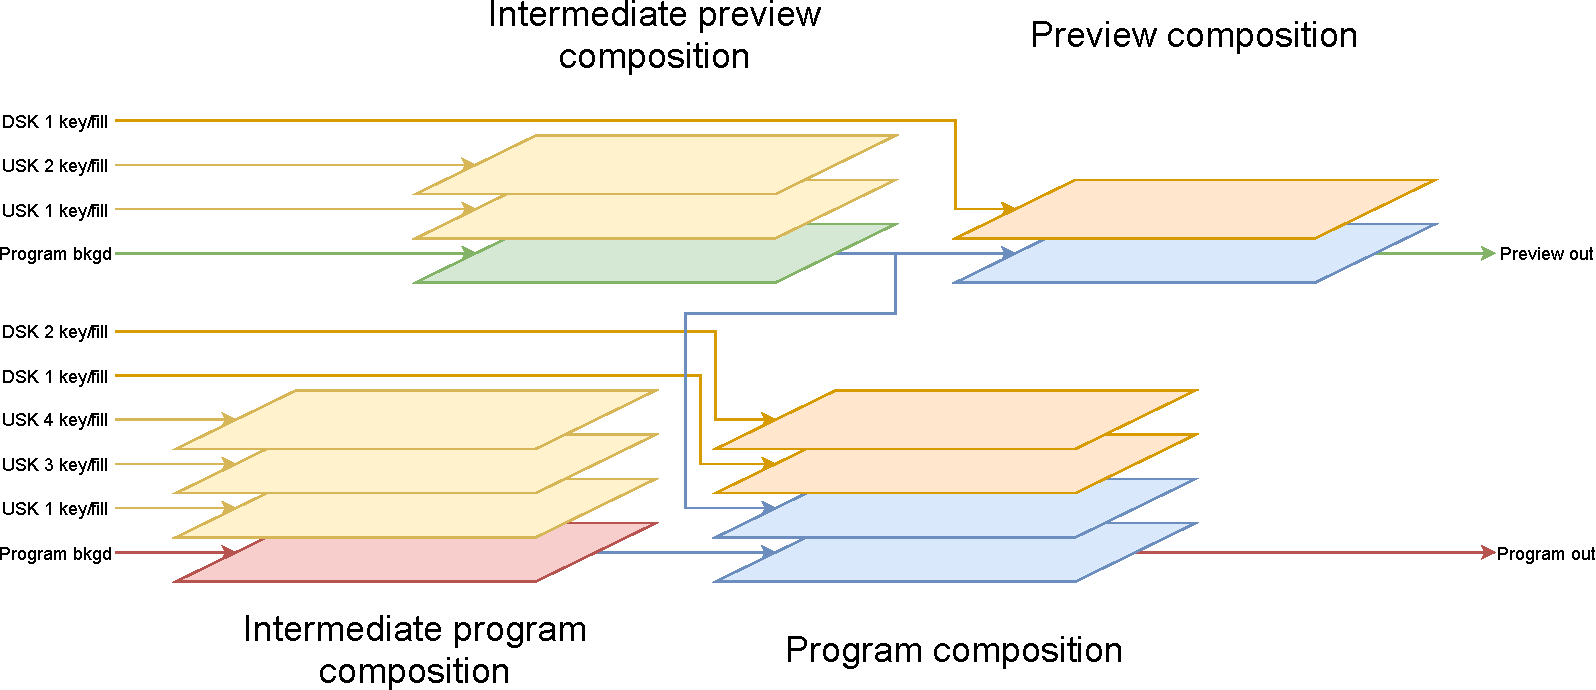
\includegraphics[width=\textwidth]{Mix effect-Transition}
    
    Layer legend: \textcolor{red}{Program background} \textcolor{green}{Preview background} \textcolor{yellow}{\glspl{usk}} \textcolor{orange}{\glspl{dsk}} \textcolor{blue}{Transition} 
    \caption{Compositing layers when a transition is in progress in the program bus}
    \label{fig:04:compositing_transition}
\end{sidewaysfigure}

\subsubsection{Overlays::Base}
This class serves as the base class for overlays. It exposes the interface required by the mix effect to perform the compositing. Currently, the only class that implements this interface is the \texttt{Keyer} but other overlays such as 3D models can be implemented to enhance the functionality of the \glspl{me}.

\subsubsection{Overlays::Keyer}
As mentioned earlier, this is the only class that implements the \texttt{Overlay} interface. This has one of the most advanced implementations, hence, it will be explained in depth later in its own section. In short terms, this allows to embed images on top of the background layer.

\subsubsection{Transitions::Base}
Similarly to the overlays, all transitions also inherit from a base class. However, the transitions are not a single layer but a collection of layers. Usually they consist of two layers, the in-coming and out-going layers. Two classes implement this interface: \texttt{Mix} and \texttt{DVE}

\subsubsection{Transitions::Mix}
This transition has both layers encompassing the whole viewport, similarly to the background layers. These two layers are progressively blended using one of the following techniques:

\begin{itemize}
    \item \textbf{Mix}: Both layers are weight-averaged using the mixing equation described on the \autoref{chap:soa}.
    \item \textbf{Add}: Both layers are added together. The first half of the transition, the foreground layer is attenuated, while in the second half, the background layer will be.
    \item \textbf{Fade}: In the first half the background layer fades out and in the second half the foreground layer fades in.
\end{itemize}

\subsubsection{Transitions::DVE}
As the name suggests, this is a \gls{dve}-based transition. Unlike the \texttt{Mix} transition, the layers used to create the \texttt{DVE} are not generally rendered full-screen. Several variations of this transition have been implemented:

\begin{itemize}
    \item \textbf{Cover}: The incoming image appears from one of the edges occluding the outgoing image. The travel direction can be determined by a continuous angle.
    \item \textbf{Uncover}: The outgoing image disappears towards one of the edges, uncovering the incoming image. The travel direction can be determined by a continuous angle.
    \item \textbf{Slide}: Both of the previous effects are executed at the same time. Therefore, it can be considered that both images move together, as if they were welded.
    \item \textbf{Rotate 3D}. The outgoing image starts rotating around a user-configured axis that is parallel to the screen. When the image is normal to the screen, the rotation continues but with the incoming image.
\end{itemize}


\subsubsection{Control::Controller}
The controller receives the commands from the \texttt{ViewBase}s. Then the \texttt{Controller} is responsible of applying the changes requested by the command, responding to the invoker \texttt{ViewBase} and broadcasting the mutations to the rest of the \texttt{ViewBase}s. These messages are interchanged as a list of strings, where each of the elements represents a token.


\subsubsection{Control::ViewBase}
A \texttt{ViewBase} represents a manner of exporting and importing commands from and to the mixer. Therefore, as mentioned earlier, it will request to the mixer mutations or queries, hear a response back and react to state changes.

\subsubsection{Control::CLIView}
This class inherits from \texttt{ViewBase} and exposes the mixer as a \gls{cli}. Therefore, its responsibility is to perform the above-mentioned tasks as a plain text interface.

\subsection{Keying}
The keying operation involves the implementation of a low-level \textit{Zuazo} component. Therefore, it is worth dedicating a section to this process. It has been implemented using a \gls{glsl} fragment shader. In the context of digital image processing, all the underlaying operations are point operations, so the keying process is also a point operation.\newline

In the figure \ref{fig:04:keyer_block_digram} it can be seen that the keyers take as input three frames. The first one is the existing contents of the framebuffer, as the resulting image will be overlayed on top of it. The second and third ones are keying and filling images. The opacity of the later one will be determined based on the former one. This opacity will be used to select between the filling image and the background according to the blending modes described earlier. This process is executed repeatedly for each keyer. The \textit{mix out} of the first one will be the \textit{background in} of the next one, and so on. The first keyer will receive as the background input the actual background layer.\newline

\begin{figure}[htbp]
    \centering
    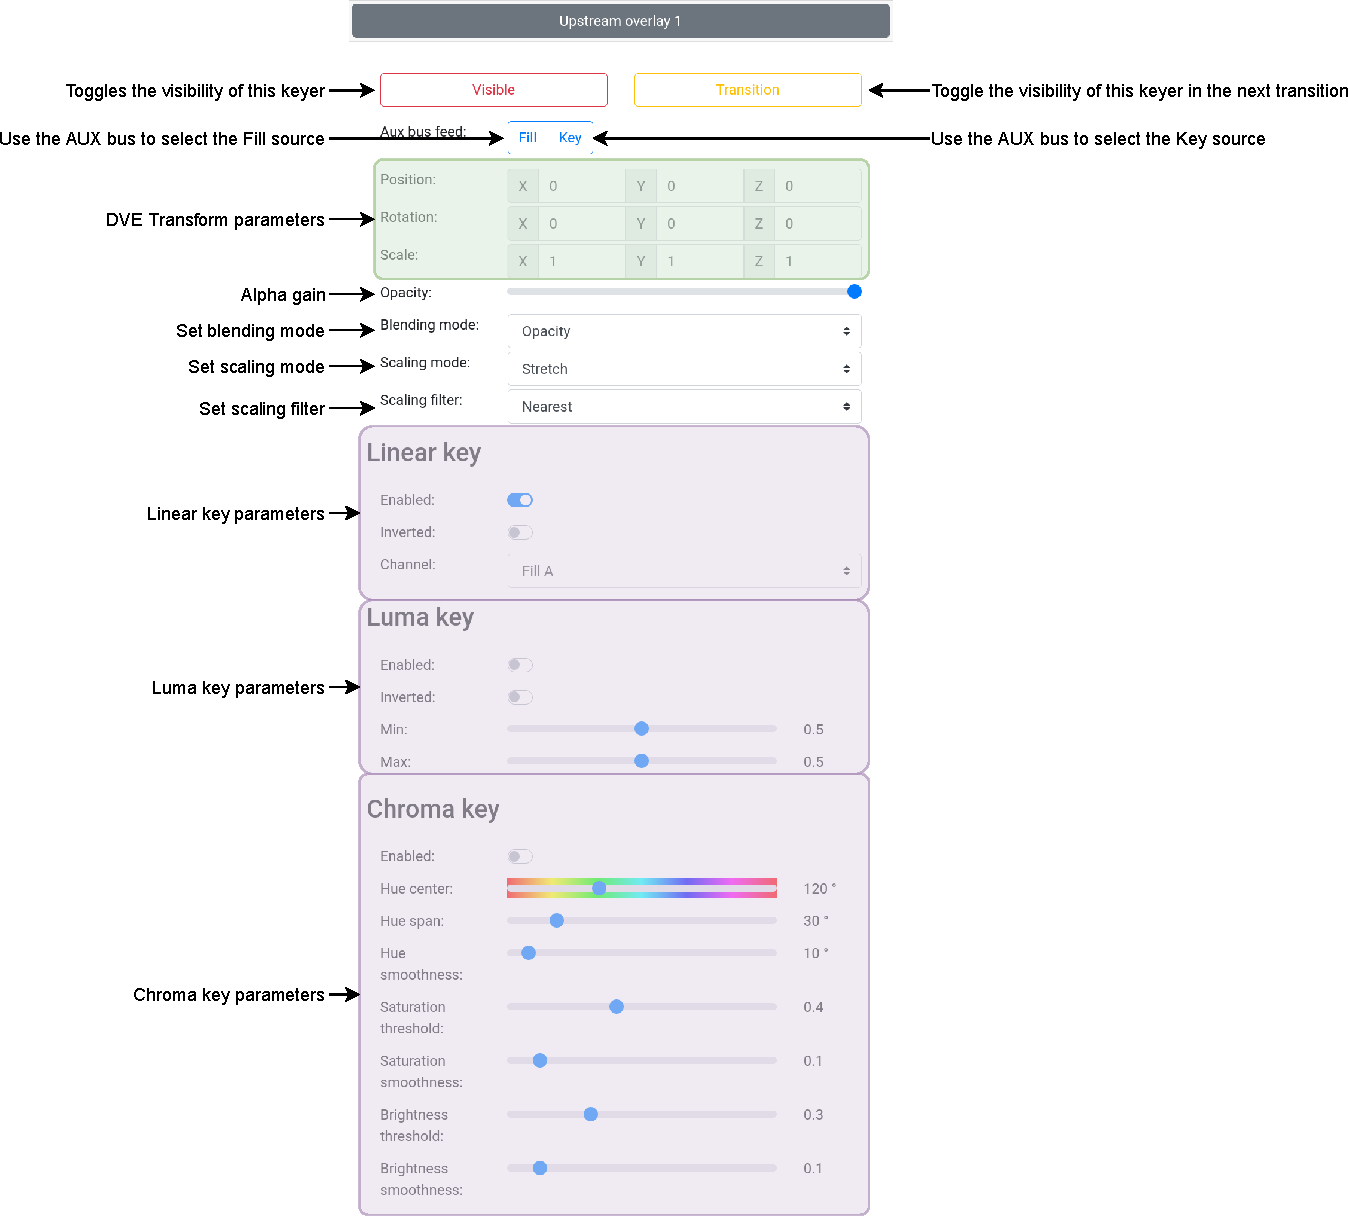
\includegraphics[width=\textwidth]{Keyer}

    \caption{Signal path of the keyer}
    \label{fig:04:keyer_block_digram}
\end{figure}

The keying signal can determine the opacity of the filling signal in the traditional three manners: Linear keying, luma keying and chroma keying. Moreover, a pattern and a global gain can also be used as the key source. These five opacity values are multiplied together and used as the $\alpha$ source in the blending stage. Any set of these five transparency sources can be used. If not enabled, it can be considered that a '$1.0$' is fed to the multiplier.\newline

\subsubsection{Linear key}
Linear keying refers to using an existing component as a transparency source for the fill signal. In this case, any of the R, G, B, A and Y components of either key or fill signals can be used as a transparency source. Moreover, the result can be complemented. As the source image is in RGB(A) colour model, in case the Y component is used, it needs to be computed according to the YUV/YIQ formula shown in the equation \eqref{eq:04:rgb2yuv_y}.\newline

\begin{equation}\label{eq:04:rgb2yuv_y}
    Y = 0.299R + 0.587G + 0.114B
\end{equation}

The most common usage would be to use the A component of the filling image when this presents an alpha channel. Moreover, if the alpha is  provided as a separate matte signal, the logical configuration would be to use the keying signal's luminance.\newline

\subsubsection{Luma key}
Luma key is very similar to a linear key configured to listen to the keying signal's luminance. Similarly to the previous keying technique, it implements an optional result complementation.\newline

The only difference with this approach is that the luminance to transparency conversion is not performed linearly. Instead, a transfer function is applied to it. This transfer function is a Hermite function, which can be configured with a lower and upper threshold, as shown in the figure \ref{fig:04:lum_transfer_function}. If $max \leq min$, this transfer function is a umbralization at $min$.\newline

\begin{figure}[htbp]
    \centering
    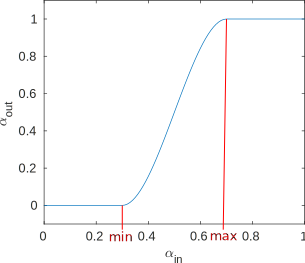
\includegraphics[width=.6\textwidth]{Luma key-Transfer}

    \caption{Luma-key's transfer function}
    \label{fig:04:lum_transfer_function}
\end{figure}




\subsubsection{Chroma key}
Chroma keying must be done in a colour model where the colour data is explicit, as this type of keying consists in using the tonality to discriminate parts of the filling image. In this case, the \gls{hsv} color model has been used. As a consequence, the first step is to convert the source pixels to this model using the equations \eqref{eq:04:rgb2hsv_hue}, \eqref{eq:04:rgb2hsv_sat} and \eqref{eq:04:rgb2hsv_val}. Although those equations may seem to be trivial to implement, they have many branches, which considerably hurts performance. Therefore, a highly optimized version written by the authors of \textit{LOLengine} has been used\cite{rgb2hsvGlsl}.\newline

\begin{equation*}
    MAX = max\{R, G, B\} \qquad MIN = min\{R, G, B\}
\end{equation*}

\begin{equation}\label{eq:04:rgb2hsv_hue}
    H = 
    \begin{cases}
        60\si{\degree} \cdot \frac{G - B}{MAX - MIN} + 0\si{\degree} & \text{if} \quad MAX=R \quad \text{and} \quad G \geq B \\
        60\si{\degree} \cdot \frac{G - B}{MAX - MIN} + 360\si{\degree} & \text{if} \quad MAX=R \quad \text{and} \quad G < B \\
        60\si{\degree} \cdot \frac{B - R}{MAX - MIN} + 120\si{\degree} & \text{if} \quad MAX=G \\
        60\si{\degree} \cdot \frac{R - G}{MAX - MIN} + 240\si{\degree} & \text{if} \quad MAX=B \\
    \end{cases}
\end{equation}

\begin{equation}\label{eq:04:rgb2hsv_sat}
    S = 
    \begin{cases}
        0 & \text{if} \quad MAX=0 \\
        1 - \frac{MIN}{MAX} & \text{otherwise}
    \end{cases}
\end{equation}

\begin{equation}\label{eq:04:rgb2hsv_val}
    V = MAX
\end{equation}

\Gls{hsv} colour model allows to easily implement the chroma key, detecting if the hue lies on a particular interval, as shown in the figure \ref{fig:04:hue_transfer_function}. This interval is configured by a central value and width. Moreover, the edges can be smoothed to steadily fade from transparent to opaque. Due to the periodicity of the hue component, the transfer function also has this nature, wrapping from $360 \si{\degree}$ back to $0 \si{\degree}$.\newline

\begin{figure}[htbp]
    \centering
    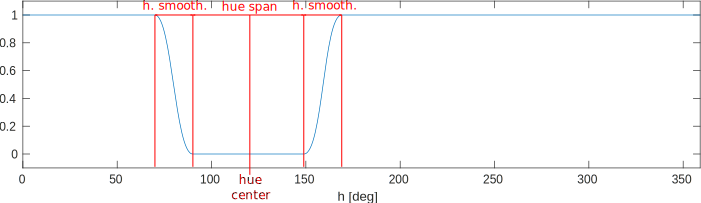
\includegraphics[width=.9\textwidth]{Chroma key-Hue transfer}

    \caption{Chroma key's hue transfer function}
    \label{fig:04:hue_transfer_function}
\end{figure}

However, the hue component is not well defined for low saturation and brightness values, as it gets very sensitive to noise. To solve this problem, a threshold is applied to the saturation and brightness components. Similarly to the hue component, this threshold can be smoothed as seen in the figures \ref{fig:04:sat_transfer_function} and \ref{fig:04:val_transfer_function}.\newline

\begin{figure}[htbp]
    \centering
    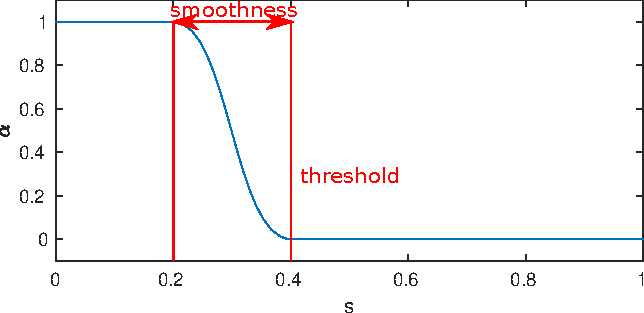
\includegraphics[width=.6\textwidth]{Chroma key-Sat transfer}

    \caption{Chroma key's saturation transfer function}
    \label{fig:04:sat_transfer_function}
\end{figure}

\begin{figure}[htbp]
    \centering
    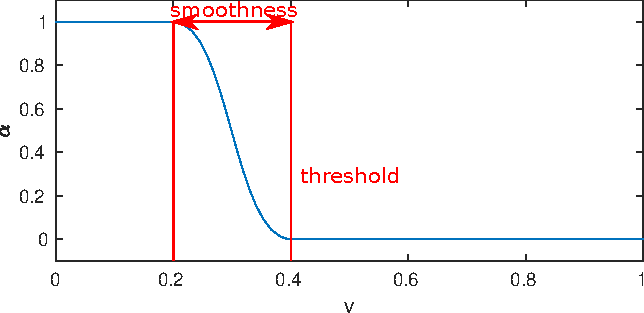
\includegraphics[width=.6\textwidth]{Chroma key-Val transfer}

    \caption{Chroma key's brightness transfer function}
    \label{fig:04:val_transfer_function}
\end{figure}

Finally, the most restrictive of the three transparency values is selected, namely, the maximum. In this way, low saturated or dark \glspl{pixel} avoid to be transparent due to the restriction imposed by the saturation and brightness transfer functions. Similarly, pure colors (maximum saturation and brightness) far away from the discriminated color will not be transparent due to the hue transfer function.\newline


\subsubsection{Pattern key}
The pattern keying can be configured to use multiple Bézier contours to crop the filling image with an arbitrary shape. This shape is completely user definable. Implementation details about the techniques used to achieve such a task are in the \autoref{chap:bezier}.\newline


\subsection{Communications}
The mixer is designed to be remotely controlled using network protocols. The control is performed using a \gls{cli}, which can be transported either over \gls{tcp} or WebSockets. The first protocol has been selected as it is widely used and it is easy to develop new applications with it. The second protocol allows interacting with web applications and works as a thin layer on top of \gls{http}, as shown in the figure \ref{fig:04:websocket}. The operation of the \gls{cli} has three principles:

\begin{figure}[htbp]
    \centering
    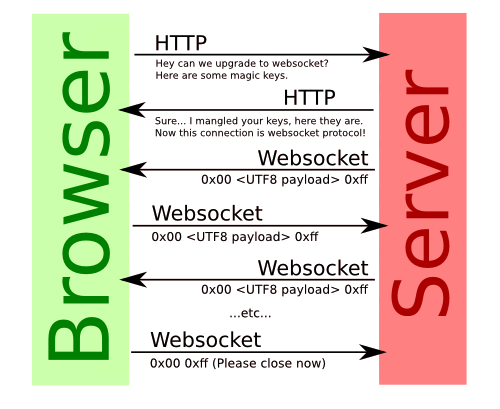
\includegraphics[width=.6\textwidth]{Websocket}

    \caption{WebSocket handshaking process}
    \label{fig:04:websocket}
\end{figure}

\begin{enumerate}
    \item Each of the commands can be considered as a chain of space separated tokens.
    \item All sent commands will receive a response from the server. This response will be either success (\texttt{OK}) or failure (\texttt{FAIL}) and may contain a tokenized payload afterwards. If a token starting with \texttt{\#} followed by a identifier is prepended to the request, this token is also prepended to the response. This allows to have multiple requests in flight.
    \item If a command mutates the state of the mixer, this command is broadcasted to all connected clients, including the invoker. However, the broadcast will suppress the identifier token.
\end{enumerate}

In-depth details about this \gls{cli} are enclosed in the mixer's manual.\newline

This control paradigm offers great flexibility for setting up multiple control environments. Some example configurations are described hereafter. Note that they are just examples and not hermetic configurations. Users may decide to vary and combine them.\newline

\subsubsection{Basic configuration}
In most cases, none of the advanced control features is used.  In this case, the server is controlled by a single client, as shown in the figure \ref{fig:04:configuration_basic}.\newline

\begin{figure}[htbp]
    \centering
    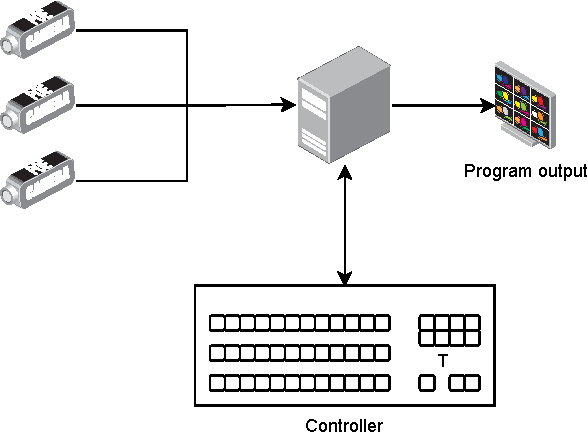
\includegraphics[width=.6\textwidth]{Configuration-Basic}

    \caption{Basic mixer control configuration}
    \label{fig:04:configuration_basic}
\end{figure}

\subsubsection{Multi-program configuration}
Some events may require to produce multiple audiovisual feeds. For instance, if a large concert is going to be broadcasted on \gls{tv}, two signals may be generated, one for \gls{tv} use and the other for image magnification inside the venue. These are usually two distinct mixes, as the image magnification feed usually focuses on close shots of the performers, while the \gls{tv} signal has more general shots. Instead of using two separate vision mixer, this task can be accomplished with a single mixer with two \gls{me} banks.\newline

However, performing two distinct mixes may overwhelm even the most experienced producers, so two producers, each one with its own controller, are required. The control mechanism allows to point each controller to each of the \glspl{me}, so they do not mess the work of each other. This configuration is displayed in the figure \ref{fig:04:configuration_multiple}.\newline

\begin{figure}[htbp]
    \centering
    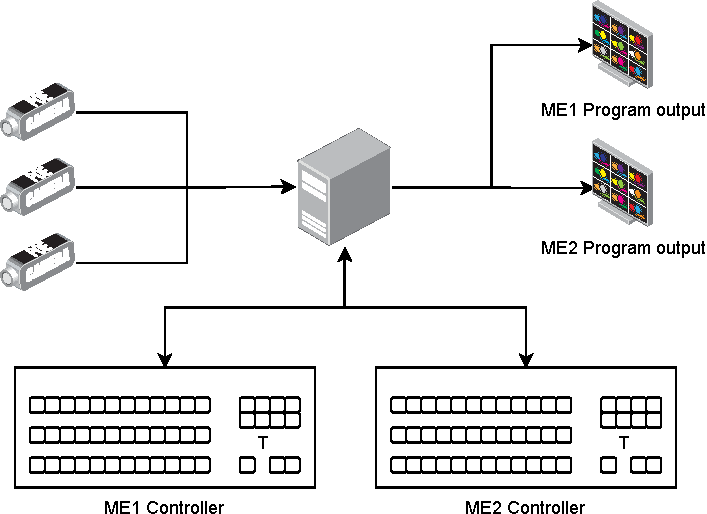
\includegraphics[width=.6\textwidth]{Configuration-Multiple}

    \caption{Multi M/E mixer control configuration}
    \label{fig:04:configuration_multiple}
\end{figure}

\subsubsection{Redundant configuration}
The last example relates to the possibility to synchronize the states of two mixers using a proxy client. This allows to implement a fail-over mechanism in case of one of the controllers or the mixers fail. This configuration is shown in the figure \ref{fig:04:configuration_redundant} and allows a catastrophic failure of any of the sides of the mirror. If this happens, the video feed will be briefly interrupted until the master switch is toggled. These switches are alien to this project, but they are commercially available.\newline

\begin{figure}[htbp]
    \centering
    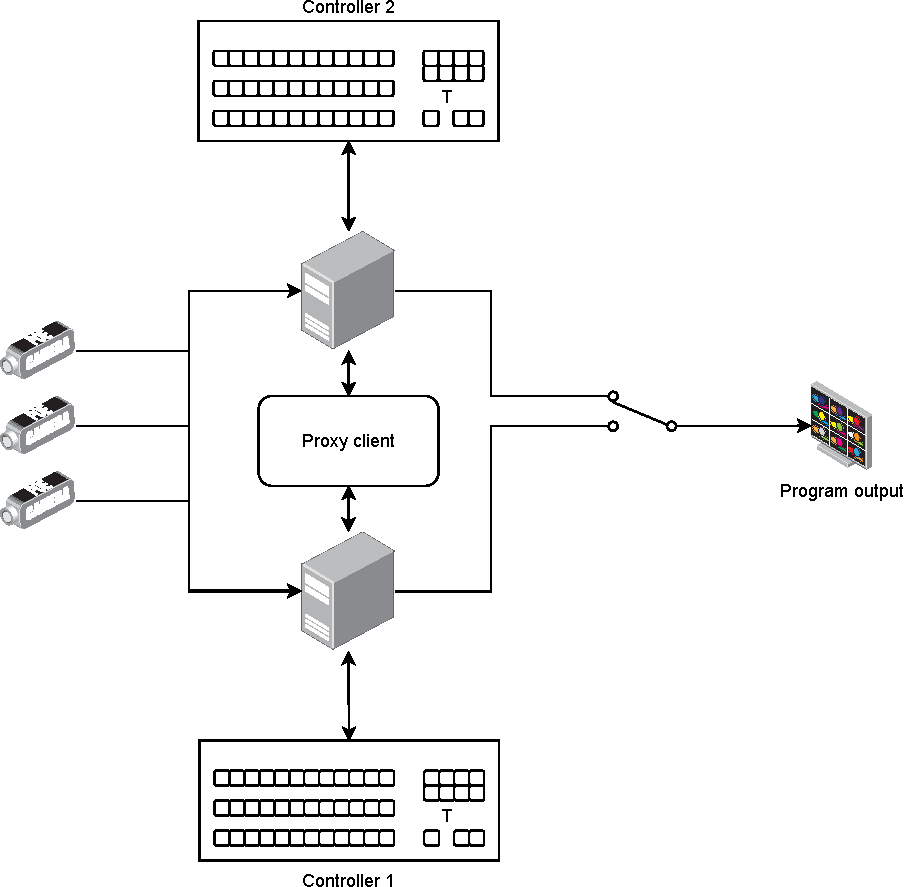
\includegraphics[width=.8\textwidth]{Configuration-Redundant}

    \caption{Redundant mixer control configuration}
    \label{fig:04:configuration_redundant}
\end{figure}



\section{Web application for control}
The main client implemented for controlling this mixer is a web application. Web applications are executed by browsers and generally do not require installation, as they are downloaded from the internet on demand. Moreover, they use interpreted programming languages, so they can be executed on any desktop platform, or even mobiles and tablets. This makes them a very versatile multi-platform development tool, and the number of web applications has sky-rocketed in the last decade. In fact, this report has been written in a web application.\newline

Web applications come with their own drawbacks. In general terms, they are not as efficient as compiled languages, making them unsuitable for compute intensive applications. However, in this case, all the heavy lifting is done in the server and the task of controlling it is very lightweight, so this concern is negligible. Another inconvenience of web applications is that they require an internet connection to work. This can be solved using \textit{Electron}, a framework to bundle web applications with an instance of \textit{Chromium} (\gls{foss} version of \textit{Google Chrome}) which serves as a standalone package of the application that works offline.\newline

This controller has been built using \textit{Vue.js} and \textit{Bootstrap} frameworks. The former one relates to the development of the \gls{ui} itself. The later one is a \gls{css} library to obtain a consistent \gls{md} look. Additionally \textit{vue-router} has been used to create multiple pages and \textit{vuex} for state management.\newline

To communicate with the server, the \gls{cli} has been implemented in \gls{js}. This commands are carried from and to the mixer using WebSockets, as this is one of the few real-time protocols widely supported by browsers. This implementation of the \gls{cli} is wrapped around a custom \textit{vuex} plugin that synchronizes the state stored in \textit{vuex} with the mixer's status.\newline

\textit{GitHub-pages} has been selected to deploy the web application, as it is free, easy to use and integrates well with the \textit{Git} version control used to develop this application. However, if desired, the resulting web page can be easily hosted in any other hosting service.\newline


%Print bibliography if it is being compiled standalone
%\printbibliography

\end{document}
